
%% bare_conf.tex
%% V1.3
%% 2007/01/11
%% by Michael Shell
%% See:
%% http://www.michaelshell.org/
%% for current contact information.
%%
%% This is a skeleton file demonstrating the use of IEEEtran.cls
%% (requires IEEEtran.cls version 1.7 or later) with an IEEE conference paper.
%%
%% Support sites:
%% http://www.michaelshell.org/tex/ieeetran/
%% http://www.ctan.org/tex-archive/macros/latex/contrib/IEEEtran/
%% and
%% http://www.ieee.org/

%%*************************************************************************
%% Legal Notice:
%% This code is offered as-is without any warranty either expressed or
%% implied; without even the implied warranty of MERCHANTABILITY or
%% FITNESS FOR A PARTICULAR PURPOSE!
%% User assumes all risk.
%% In no event shall IEEE or any contributor to this code be liable for
%% any damages or losses, including, but not limited to, incidental,
%% consequential, or any other damages, resulting from the use or misuse
%% of any information contained here.
%%
%% All comments are the opinions of their respective authors and are not
%% necessarily endorsed by the IEEE.
%%
%% This work is distributed under the LaTeX Project Public License (LPPL)
%% ( http://www.latex-project.org/ ) version 1.3, and may be freely used,
%% distributed and modified. A copy of the LPPL, version 1.3, is included
%% in the base LaTeX documentation of all distributions of LaTeX released
%% 2003/12/01 or later.
%% Retain all contribution notices and credits.
%% ** Modified files should be clearly indicated as such, including  **
%% ** renaming them and changing author support contact information. **
%%
%% File list of work: IEEEtran.cls, IEEEtran_HOWTO.pdf, bare_adv.tex,
%%                    bare_conf.tex, bare_jrnl.tex, bare_jrnl_compsoc.tex
%%*************************************************************************

% *** Authors should verify (and, if needed, correct) their LaTeX system  ***
% *** with the testflow diagnostic prior to trusting their LaTeX platform ***
% *** with production work. IEEE's font choices can trigger bugs that do  ***
% *** not appear when using other class files.                            ***
% The testflow support page is at:
% http://www.michaelshell.org/tex/testflow/

\documentclass[10pt,conference,a4paper]{argencon}

\usepackage[latin1]{inputenc}
\usepackage[compress]{cite}
\usepackage{graphicx}

% Para que el t�tulo referencias aparezca en espa�ol puede usar la siguiente sentencia
% \renewcommand{\refname}{Referencias}

% correct bad hyphenation here
\hyphenation{op-tical net-works semi-conduc-tor}


\begin{document}

% paper title
% can use linebreaks \\ within to get better formatting as desired
\title{Sample ARGENCON Paper for A4 Page Size}

\author{\IEEEauthorblockN{First Author\IEEEauthorrefmark{2}$^1$, Second Author\IEEEauthorrefmark{1}$^2$ and Third Author\IEEEauthorrefmark{2}$^3$\vspace{0.2cm}}\IEEEauthorblockA{\IEEEauthorrefmark{2}\emph{First-Third Department, First-Third University}\\\emph{Address Including Country Name}}\IEEEauthorblockA{$^1$\texttt{\small{first.author@first-third.edu}}\\$^3$\texttt{\small{third.author@first-third.edu}}}\IEEEauthorblockA{\IEEEauthorrefmark{1}\emph{Second Company}\\\emph{Address Including Country Name}\\$^2$\texttt{\small{second.author@second.com}}}}

% conference papers do not typically use \thanks and this command
% is locked out in conference mode. If really needed, such as for
% the acknowledgment of grants, issue a \IEEEoverridecommandlockouts
% after \documentclass

% use for special paper notices
%\IEEEspecialpapernotice{(Invited Paper)}

% make the title area
\maketitle

\begin{abstract}
%\boldmath
For your paper to be published in the conference proceedings, you must use this document as both an instruction set and as a template into which you can type your own text.  If your paper does not conform to the required format, you will be asked to fix it. Note that the abstract should be written both in English and Spanish.
\\
\\
$~~$\emph{Resumen---} Para que su trabajo sea publicado en las actas del congreso debe usar este documento como instructivo y como plantilla sobre al cual basar su propio texto. Si su trabajo no respeta el formato requerido se le solicitar� su adecuaci�n. Note que el resumen debe escribirse tanto en ingl�s como en espa�ol.
\end{abstract}

% no keywords

\IEEEpeerreviewmaketitle

\section{Introduction}
% no \IEEEPARstart
This document is a template.  An electronic copy can be downloaded from the conference website.  For questions on paper guidelines, please contact the conference publications committee as indicated on the conference website.  Information about final paper submission is available from the conference website.
Before submitting your final paper, check that the format conforms to this template.  Specifically, check the appearance of the title and author block, the appearance of section headings, document margins, column width, column spacing and other features.

\subsection{This Sub-Section for LaTeX Users Only}
This demo file is intended to serve as a ``starter file'' for IEEE conference papers produced under \LaTeX\ using IEEEtran.cls version 1.7 and later.

If the appearance is different from what is shown in this template, then the cause may be the use of conflicting style files in your LaTeX document.  An example of an incompatible style file is latex8.sty.  You must remove all such conflicting style files.

\section{Page layout}
An easy way to comply with the conference paper formatting requirements is to use this document as a template and simply type your text into it.

\subsection{Page layout}
Your paper must use a page size corresponding to A4 which is 210 mm wide and 297 mm long.  The margins must be set as follows:
\begin{itemize}
  \item Top = 19 mm (0.75")
  \item Bottom = 25.4 mm (1")
  \item Left = Right = 17.3 mm (0.68")
\end{itemize}
Your paper must be in two column format with a space of 4.22 mm (0.17") between columns.

\section{Page style}
All paragraphs must be indented.  All paragraphs must be justified, i.e. both left-justified and right-justified.

\subsection{Text Font of Entire Document}
The entire document should be in Times New Roman or Times font.  Type 3 fonts must not be used.  Other font types may be used if needed for special purposes.
Recommended font sizes are shown in Table \ref{TAB: fonts}.

\subsection{Title and Author Details
\label{SUBSEC: title and authors}}
Title must be in 24 pt Regular font.  Author name must be in 11 pt Regular font.  Author affiliation must be in 10 pt Italic.  Email address must be in 9 pt Courier Regular font.

\begin{table}[h]
\centering
\caption{Font sizes for papers.}
\begin{tabular}{|p{0.05\columnwidth}|p{0.35\columnwidth}|p{0.15\columnwidth}|p{0.25\columnwidth}|} \hline
\textbf{Font} & \multicolumn{3}{|c|}{\textbf{Appearance (in Time New Roman or Times)}} \\ \cline{2-4}
\textbf{Size} & \textbf{Regular} & \textbf{Bold} & \textbf{Italic} \\ \hline
8 & table caption (in Small Caps), figure caption, reference item & & reference item (partial) \\ \hline
9 & author email address (in Courier), cell in a table & abstract body & abstract heading (also in Bold) \\ \hline
10 & level-1 heading (in Small Caps), paragraph & & level-2 heading, level-3 heading, author affiliation \\ \hline
11 & author name & & \\ \hline
24 & title & & \\ \hline
\end{tabular}
\label{TAB: fonts}
\end{table}

All title and author details must be in single-column format and must be centered.

Every word in a title must be capitalized except for short minor words such as ``a'', ``an'', ``and'', ``as'', ``at'', ``by'', ``for'', ``from'', ``if'', ``in'', ``into'', ``on'', ``or'', ``of'', ``the'', ``to'', ``with''.

Author details must not show any professional title (e.g. Managing Director), any academic title (e.g. Dr.) or any membership of any professional organization (e.g. Senior Member IEEE).

To avoid confusion, the family name must be written as the last part of each author name (e.g. John A.K. Smith).
Each affiliation must include, at the very least, the name of the company or institute  and the name of the country where the author is based.

Email address is compulsory for the corresponding author.

\subsection{Section Headings}

No more than 3 levels of headings should be used.  All headings must be in 10 pt font.  Every word in a heading must be capitalized except for short minor words as listed in Section \ref{SUBSEC: title and authors}.

\subsubsection{Level-1 Heading}
A level-1 heading must be in Small Caps, centered and numbered using uppercase Roman numerals.  For example, see heading ``III. Page Style'' of this document.  The two level-1 headings which must not be numbered are ``Acknowledgment'' and ``References''.

\subsubsection{Level-2 Heading}
A level-2 heading must be in Italic, left-justified and numbered using an uppercase alphabetic letter followed by a period.  For example, see heading ``C. Section Headings'' above.

\subsubsection{Level-3 Heading}
A level-3 heading must be indented,  in Italic and numbered with an Arabic numeral followed by a right parenthesis. The level-3 heading must end with a colon.  The body of the level-3 section immediately follows the level-3 heading in the same paragraph.  For example, this paragraph begins with a level-3 heading.

\subsection{Equations}

Equations must be centered in the column
\begin{equation}
\dot{x}=f_{1}\left( x_{1},t\right) +\alpha x_{2}\sin \left( \theta \right),
\label{EQ: eq 1}
\end{equation}
they must be numbered using Arabic numerals and the equation number must be placed aligned along the right margin, as shown in Eq. (\ref{EQ: eq 1}).

\subsection{Figures and Tables}
Figures and tables must be centered in the column.  Large figures and tables may span across both columns.  Any table or figure that takes up more than 1 column width must be positioned either at the top or at the bottom of the page.
Graphics may be full color.  All colors will be retained on the CDROM.  Graphics must not use stipple fill patterns because they may not be reproduced properly.  Please use only SOLID FILL colors which contrast well both on screen and on a black-and-white hardcopy, as shown in Fig. \ref{FIG: figura 1}.

\begin{figure}[!h]
\centering
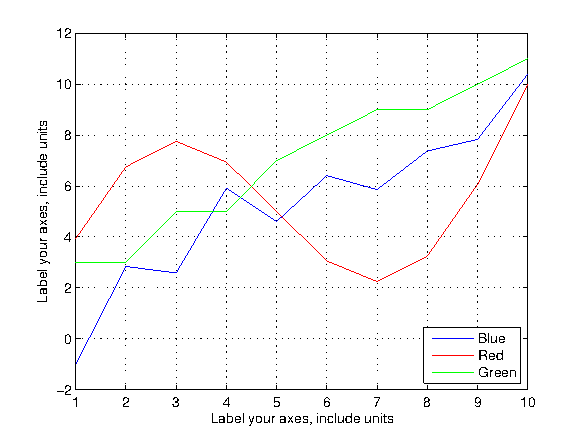
\includegraphics[clip,width=0.95\columnwidth]{grafico.png}
\caption{A sample line graph using colors which contrast well both on screen and on a black-and-white hardcopy.}
\label{FIG: figura 1}
\end{figure}

Fig. \ref{FIG: figura 2} shows an example of a low-resolution image which would not be acceptable, whereas Fig. \ref{FIG: figura 3} shows an example of an image with adequate resolution.  Check that the resolution is adequate to reveal the important detail in the figure.

Please check all figures in your paper both on screen and on a black-and-white hardcopy.  When you check your paper on a black-and-white hardcopy, please ensure that:
\begin{itemize}
  \item the colors used in each figure contrast well,
  \item the image used in each figure is clear,
  \item all text labels in each figure are legible.
\end{itemize}

\begin{figure}[!h]
\centering
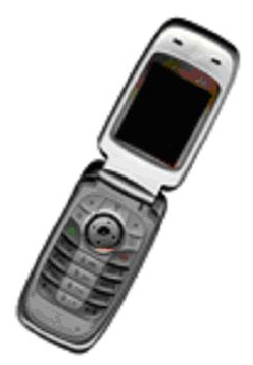
\includegraphics[clip,width=0.5\columnwidth]{mala.png}
\caption{Example of an unacceptable low-resolution image.}
\label{FIG: figura 2}
\end{figure}

\begin{figure}[!h]
\centering
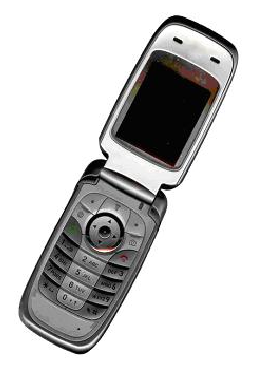
\includegraphics[clip,width=0.5\columnwidth]{buena.png}
\caption{Example of an image with acceptable resolution.}
\label{FIG: figura 3}
\end{figure}

\subsection{Figure Captions}
Figures must be numbered using Arabic numerals.  Figure captions must be in 8 pt Regular font.  Captions of a single line (e.g. Fig. \ref{FIG: figura 2}) must be centered whereas multi-line captions must be justified (e.g. Fig. \ref{FIG: figura 1}).  Captions with figure numbers must be placed after their associated figures, as shown in Fig. \ref{FIG: figura 1}.

\subsection{Table Captions}
Tables must be numbered using uppercase Roman numerals.  Table captions must be centred and in 8 pt Regular font with Small Caps.  Every word in a table caption must be capitalized except for short minor words as listed in Section \ref{SUBSEC: title and authors}.  Captions with table numbers must be placed before their associated tables, as shown in Table \ref{TAB: fonts}.

\subsection{Page Numbers, Headers and Footers}
Page numbers, headers and footers must not be used.

\subsection{Links and Bookmarks}
All hypertext links and section bookmarks will be removed from papers during the processing of papers for publication.  If you need to refer to an Internet email address or URL in your paper, you must type out the address or URL fully in Regular font.

\subsection{References}
The heading of the References section must not be numbered.  All reference items must be in 8 pt font.  Please use Regular and Italic styles to distinguish different fields as shown in the References section.  Number the reference items consecutively in square brackets (e.g. \cite{IEEEexample:book}).
When referring to a reference item, please simply use the reference number, as in \cite{IEEEexample:bookwithseriesvolume}.  Do not use ``Ref. \cite{IEEEexample:article_typical}'' or ``Reference \cite{IEEEexample:article_typical}'' except at the beginning of a sentence, e.g.  ``Reference \cite{IEEEexample:article_typical} shows ...''.  Multiple references are each numbered with separate brackets (e.g. \cite{IEEEexample:bookwithseriesvolume}, \cite{IEEEexample:article_typical}, \cite{IEEEexample:confwithpaper,IEEEexample:uspat,IEEEexample:IEEEwebsite}).
Examples of reference items of different categories shown in the References section include:
\begin{itemize}
  \item example of a book in \cite{IEEEexample:book}
  \item example of a book in a series in \cite{IEEEexample:bookwithseriesvolume}
  \item example of a journal article in \cite{IEEEexample:article_typical}
  \item example of a conference paper in \cite{IEEEexample:confwithpaper}
  \item example of a patent in \cite{IEEEexample:uspat}
  \item example of a website in \cite{IEEEexample:IEEEwebsite}
  \item example of a web page in \cite{IEEEhowto:IEEEtranpage}
  \item example of a databook as a manual in \cite{IEEEexample:motmanual}
  \item example of a datasheet in \cite{IEEEexample:datasheet}
  \item example of a master's thesis in \cite{IEEEexample:masterstype}
  \item example of a technical report in \cite{IEEEexample:techreptype}
  \item example of a standard in \cite{IEEEexample:standard}
\end{itemize}


\section{Conclusion}
The LaTeX templates depend on the official IEEEtran.cls and IEEEtran.bst files, whereas the Microsoft Word templates are self-contained.

% conference papers do not normally have an appendix

% use section* for acknowledgement
\section*{Acknowledgment}
The heading of the Acknowledgment section and the References section must not be numbered.
We wish to acknowledge Michael Shell and other contributors for developing and maintaining the IEEE LaTeX style files which have been used in the preparation of this template.  To see the list of contributors, please refer to the top of file IEEETran.cls in the IEEE LaTeX distribution.

% references section

% can use a bibliography generated by BibTeX as a .bbl file
% BibTeX documentation can be easily obtained at:
% http://www.ctan.org/tex-archive/biblio/bibtex/contrib/doc/
% The IEEEtran BibTeX style support page is at:
% http://www.michaelshell.org/tex/ieeetran/bibtex/
%\bibliographystyle{IEEEtran}
% argument is your BibTeX string definitions and bibliography database(s)
%\bibliography{IEEEabrv,../bib/paper}
%
% <OR> manually copy in the resultant .bbl file
% set second argument of \begin to the number of references
% (used to reserve space for the reference number labels box)

\bibliographystyle{IEEEtran}
\bibliography{IEEEexample}

% that's all folks
\end{document}


